

\chapter{Estudo de Caso}

Neste capítulo é apresentado o estudo de caso, onde os dados públicos do programa Bolsa Família são inseridos e extraídos de um banco de dados não relacional Cassandra, com \emph{clusters} de um, dois, quatro e seis máquinas, além das descrições das etapas e programas utilizados. O programa é exposto brevemente e o modelo de dados e o ambiente utilizado são descritos.

\section{O Programa Bolsa Família}
O Bolsa Família é um programa federal, em operação desde 2003 quando foi instituído pelo então presidente Luiz Inácio Lula da Silva, com objetivo de "combater a fome e promover a segurança alimentar e nutricional, combater a pobreza e outras formas de privação das famílias e promover o acesso à rede de serviços públicos, em especial, saúde, educação, segurança alimentar e assistência social"~\cite{caixa-bolsafamilia}. 
O programa se caracteriza pela transferência de renda para famílias brasileiras em situação de pobreza e extrema pobreza, ou seja, que recebam até R\$170 e R\$85 respectivamente. Atualmente cerca de 13,9 milhões de famílias são atendidas pelo programa, recebendo em média R\$182 cada, totalizando R\$27,4 bilhões em 2016, que recebem recursos do Ministério do Desenvolvimento Social, por meio da Caixa Econômica Federal~\cite{gov-bolsafamilia1, gov-bolsafamilia2}.

Os dados do Bolsa Família utilizados para estudo de caso nesse trabalho foram obtidos no \emph{site} do Portal da Transparência, um projeto da Controladoria Geral da União, que disponibiliza informações sobre os gastos do dinheiro público, com objetivo de melhorar a transparência da gestão pública~\cite{sobreportaldatransparencia}. 

Esses dados são disponibilizados em formato aberto \emph{.csv}, e agrupados mensalmente, trazendo informações sobre a transferência de recursos federais aos participantes do programa. 

\subsection{Dados Utilizados}

Para os testes de desempenho foram utilizados um total de trinta arquivos, correspondentes a trinta meses do programa, compreendidos entre Julho de 2014 e Dezembro de 2016. O total de arquivos foi determinado considerando-se a capacidade de capacidade de armazenamento das máquinas do ambiente utilizado, especialmente nos testes de \emph{cluster} com apenas duas máquinas. Cada arquivo utilizado possui em média 16GiB de tamanho e 13.968.749 registros.

Cada arquivo apresenta como campos: \textbf{UF, Código SIAFI Município, Nome Município, Código Função, Código Subfunção, Código Programa, Código Ação, NIS Favorecido, Nome Favorecido, Fonte-Finalidade, Valor Parcela e Mês Competência}. Como os testes realizados não buscam a análise e interpretação dos dados armazenados, e sim uma mensurar uma possível melhora de desempenho, um subconjunto dessas colunas foi escolhido para a realização desse trabalho. A tabela \ref{tab:colunas} apresenta os campos presentes nos arquivos, bem como seus tipos e quais campos foram utilizados na modelagem dos dados.

\begin{table}[]
	\centering
	\caption{Campos utilizados}
	\label{tab:colunas}
	\begin{tabular}{|l|c|c|}
		\hline
		\textbf{Campo}         & \textbf{Tipo} & \textbf{Utilizado} \\ \hline
		UF                     & Text          & Sim                \\ \hline
		Código SIAFI Município & Int           & Sim                \\ \hline
		Nome Município         & Text          & Sim                \\ \hline
		Código Função          & -             & Não                \\ \hline
		Código Subfunção       & -             & Não                \\ \hline
		Código Programa        & -             & Não                \\ \hline
		Código Ação            & -             & Não                \\ \hline
		NIS Favorecido         & Bigint        & Sim                \\ \hline
		Nome Favorecido        & Text          & Sim                \\ \hline
		Fonte-Finalidade       & Text          & Sim                \\ \hline
		Valor Parcela          & Double        & Sim                \\ \hline
		Mês Competência        & Timestamp     & Sim                \\ \hline
	\end{tabular}
\end{table}

\section{Modelo de dados Cassandra}
O modelo de dados do Cassandra foi criado utilizando-se um \emph{keyspace} com fator de replicação de apenas um. O código ~\ref{lst:cql_create_keyspace} apresenta o comando CLQ utilizado para sua criação. O fator de replicação foi definido considerando que a tolerância a falhas não é um fator relevante nos testes a serem realizados, devido ao ambiente controlado em que eles são feitos.

O Cassandra apresenta duas estratégias de replicações de dados, a \emph{SimpleStrategy} e a \emph{NetworkTopologyStrategy}, sendo a primeira utilizada em \emph{datacenters} únicos e com apenas um \emph{rack}, e a segunda para uso em múltiplos \emph{datacenters}. Devido ao ambiente restrito do laboratório utilizado, foi escolhida a \emph{SimpleStrategy} como estratégia de replicação dos dados.

\noindent
\begin{minipage}[c]{1\textwidth}
\begin{lstlisting}[caption={Código CQL para criação do keyspace},label={lst:cql_create_keyspace},language=SQL]
CREATE KEYSPACE bolsa_familia WITH replication = {'class': 'SimpleStrategy', 'replication_factor': 1};
\end{lstlisting}
\end{minipage}

Apenas uma tabela foi utilizada para os testes, contendo as colunas definidas anteriormente. O código ~\ref{lst:cql_create_table} apresenta o comando CQL utilizado para sua criação.

\noindent
\begin{minipage}[c]{1\textwidth}
	\begin{lstlisting}[caption={Código CQL para criação da tabela},label={lst:cql_create_table},language=SQL]
	CREATE TABLE bolsa_familia.dados (uf TEXT, periodo TIMESTAMP, valor DOUBLE, nis_favorecido BIGINT, cod_municipio INT, fonte TEXT, nome_favorecido TEXT, nome_municipio TEXT, PRIMARY KEY(nis_favorecido, periodo, valor));
	\end{lstlisting}
\end{minipage}

Ao se definir uma chave primária no Cassandra é necessária a escolha de uma \emph{Partition Key} (chave de partição) e uma \emph{Clustering Key} (chave de agrupamento). A \emph{Partition Key} é responsável pela distribuição dos dados nos nós do ambiente, enquanto a \emph{Clustering Key} distribui esses dados dentro de cada nó.

Para determinar a localização de um registro dentro do \emph{cluster}, o particionador utilizado realiza um processo de \emph{hash} na chave de partição, sendo recomendável, então, a escolha de uma chave de partição que apresente boa distribuição dos dados dentro do \emph{cluster}. 

Para isso foi utilizada a coluna \textbf{nis\_favorecido}, por ser ela a responsável por identificar unicamente cada beneficiário do programa. Além disso, para complementar a chave primária foram escolhidos os campos \textbf{Valor Parcela e Mês Competência}, que identificam unicamente cada registro, considerando que um mesmo favorecido pelo programa(identificado pela coluna NIS Favorecido), pode receber mais de uma parcela em um mesmo mês, ou parcelas em meses distintos. A figura \ref{fig:modelocassandra} traz o modelo utilizado, onde são apresentadas as chaves primárias, separadas em chave de partição e de agrupamento, e as demais colunas que são definidas por elas.

\begin{figure}[!htb]
	\centering
	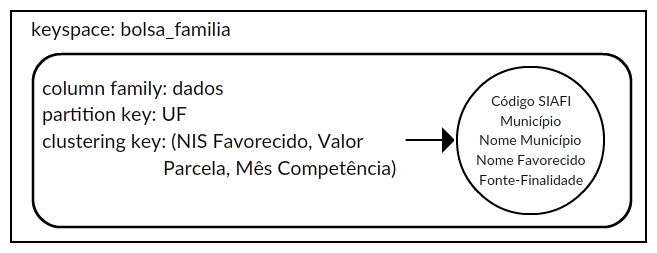
\includegraphics[width=1\textwidth]{figuras/modelocassandra.png}
	\caption{Modelo de Dados}
	\label{fig:modelocassandra}
\end{figure}

A configuração do ambiente Cassandra foi feita por meio do cliente \emph{cqlsh}, que permite a realização de consultas e manipulações no banco por meio da linguagem \emph{CQL}(\emph{Cassandra Query Language}).

\section{Arquitetura do Ambiente}
O ambiente utilizado consiste em um \emph{cluster} composto por seis máquinas com Intel i5-4570 3.20GHz, 16GB de RAM, disco rígido de 500GB, com sistema operacional Ubuntu, como representado na figura~\ref{fig:ambiente}.

\begin{figure}[!htb]
	\centering
	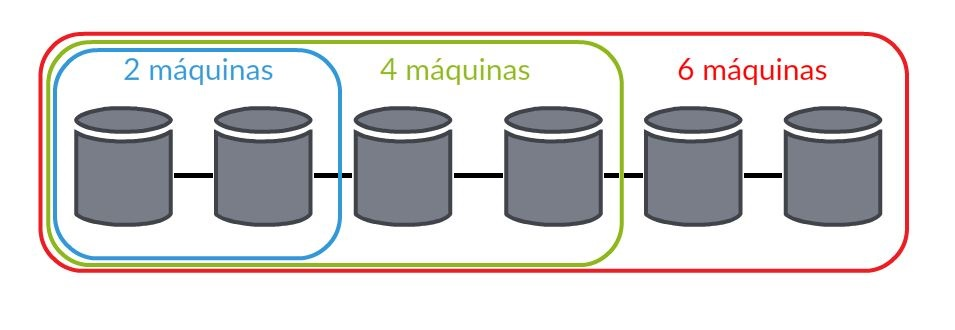
\includegraphics[width=1\textwidth]{figuras/ambiente.jpg}
	\caption{Ambiente utilizado}
	\label{fig:ambiente}
\end{figure}

O cliente Cassandra, em sua versão 3.0.4, foi instalado em cada uma das seis máquinas utilizadas no teste.

Em cada máquina foi necessária a modificação do arquivo de configuração \emph{cassandra.yaml} para possibilitar correta configuração e detecção do \emph{cluster}. O número de nós virtuais foi mantido em 256, valor recomendado para manter um balanceamento correto dos nós, o particionador padrão \emph{Murmur3Partitioner} foi mantido por ser o recomendado para novos \emph{clusters}~\cite{cassandrapartitioners}, e como \emph{snitch} foi utilizado o \emph{SimpleSnitch}, pois a implementação desenvolvida faz uso de apenas um \emph{datacenter}. 

O arquivo \emph{cassandra.yaml} também define os IPs dos nós \emph{seed}, responsáveis por manter informações sobre os outros nós, bem como o nome do \emph{cluster} utilizado. Esses dados devem ser configurados de forma idêntica em todos as máquinas para permitir a sua detecção dentro do mesmo \emph{cluster}. A configurações definidas no arquivo são apresentadas em ~\ref{lst:yaml}.

\begin{lstlisting}[caption={Configuração cassandra.yaml},label={lst:yaml},language=python]
cluster_name: 'BolsaFamilia Cluster C2M FR1'

num_tokens: 256

partitioner: org.apache.cassandra.dht.Murmur3Partitioner

seed_provider:
	- class_name: org.apache.cassandra.locator.SimpleSeedProvider
	parameters:
		- seeds: "164.41.40.35"

endpoint_snitch: SimpleSnitch

\end{lstlisting}

Além disso, seguindo as orientações em ~\cite{cassandrasettings}, e guardadas as devidas limitações do laboratório, foram realizadas as configurações do Linux:
\begin{itemize}
	\item Remoção do limite de memória (parâmetro \emph{memlock})
	\item Aumento do limite do número de arquivos abertos(parâmetro \emph{nofile})
	\item Desativação do \emph{swap}
\end{itemize}

\section{Desenvolvimento da aplicação}
Para inserção e busca dos dados no ambiente, foi desenvolvida uma aplicação em Java utilizando o \emph{driver} oferecido pela \emph{Datastax}, empresa que disponibiliza um distribuição gratuita do Apache Cassandra. Essa aplicação é responsável pela leitura de todos os arquivos de entrada e inserção dos campos utilizados no banco de dados Cassandra, assim como a posterior busca desses dados.

A inserção dos dados é feita de forma assíncrona utilizando os métodos do \emph{driver}. O tratamento dos campos utilizados é feita no momento da inserção pelo próprio programa desenvolvido. Essa filtragem é responsável pela separação dos campos das linhas do arquivo .csv utilizado, bem como a seleção dos campos que serão utilizados na análise. 

A leitura dos dados é feita no mesmo programa, após a inserção de todos os dados, também utilizando o driver da \emph{Datastax}.

Todas as interações com o banco, seja na inserção quanto na leitura, foram realizadas por meio da linguagem CQL, que se assemelha a consultas padrões SQL.



